\subsection{Kortslutningssikring}
\label{effekt_kortslutningssikring}
Kortslutningssikringen tilføjes ved at indføre kredsløbet, vist på figur \ref{fig:dia-kortslut}, mellem base og emitter på darlingtontransistorerne, belastningen og tilbagekoblingen, som vist på figur \ref{fig:dia-kortslut1}. 

\begin{figure}[h]
\centering
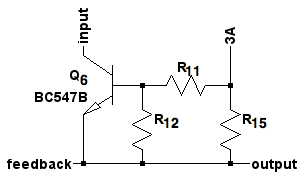
\includegraphics[scale=0.5]{teknisk/effektforstaerker/diagram-kortslut.png}
\caption{Overordnet diagram over kortslutningssikringens aktiveringssituation}
\label{fig:dia-kortslut}
\end{figure}

Strømmen på 3 A, anført på figur \ref{fig:dia-kortslut}, er den strøm, hvor kortslutningssikringen skal aktivere, hvilket blev bestemt i afsnit \ref{valg_kortslutningssikring}. At kortslutningssikringen skal aktivere betyder her, at transistoren Q1 skal åbnes. Når transistoren, Q1, åbnes vil den trække en strøm, hvormed strømmen ind i darlingtontransistorens base går mod nul og darlingtontransistoren lukker. 

\begin{figure}[h]
\centering
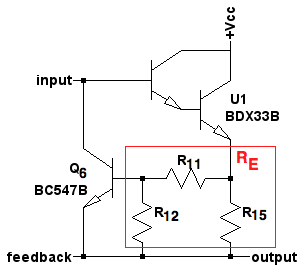
\includegraphics[scale=0.5]{teknisk/effektforstaerker/diagram-kortslut1.png}
\caption{Overordnet diagram over kortslutningssikring forbundet darlingtontransistor}
\label{fig:dia-kortslut1}
\end{figure}

Modstandene $R_{11}$, $R_{12}$ og $R_{15}$ skal, som vist på figur \ref{fig:dia-kortslut1}, repræsentere samme modstandsværdi som $R_E$, som blev beregnet i afsnit \ref{effekt_stroemforstaerker}, da den stadig skal sikre termisk stabilitet. For at åbne Q1 skal der, ifølge databladet for en BC547B \cite{bc547b-datablad}, være en base-emitter spænding på 720 mV \fixme{Jonas- Åbner den ikke lidt før?}, hvilket vil sige spændingen over $R_{12}$ skal være 720 mV når der løber 3 A fra darlingtontransistorens emitter. Dermed er det muligt at opstille de to udtryk vist formel (\ref{equ:kortslut-betingelse}) og i formel (\ref{equ:kortslut-betingelse1}) til bestemmelse af de tre modstande.

\begin{equation}
\label{equ:kortslut-betingelse}
\mathrm{536~m\ohm} = \frac{1}{\frac{1}{R_{15}}+\frac{1}{R_{11} + R_{12}}}
\end{equation}

\begin{equation}
\label{equ:kortslut-betingelse1}
\mathrm{720~mV} = R_{12} \cdot \frac{R_{15} \cdot \mathrm{3~A}}{R_{11} + R_{12} + R_{15}}
\end{equation}

Det vides desuden, at modstanden af en parallelkobling af modstande er mindre end modstanden af den mindste gren i parallelkoblingen. Dermed vælges $R_{15}$ til den mindste tilgængelige effektmodstand, som er større end den beregnede $R_E$ modstand. Størrelsen på $R_{15}$ er derfor 0,68~\ohm, hvorved $R_{11}$ og $R_{12}$ kan bestemmes til henholdsvis 1,40~\ohm~ og 1,13~\ohm. Effekten afsat i en modstand kan bestemmes som $P = I^2 \cdot R$, hvorved effekten afsat i hver enkelt af de tre modstande $R_{15}$, $R_{11}$ og $R_{12}$ kan bestemmes som vist i henholdsvis formel (\ref{equ:pr1}), formel (\ref{equ:pr2}) og formel (\ref{equ:pr3}).

\begin{equation}
\label{equ:pr1}
P_{R_{15}} = \left(\frac{(R_{11} + R{12}) \cdot \mathrm{3~A}}{R_{15} + R_{11} + R_{12}}\right)^2 \cdot R_{15} = \mathrm{3,80~W}
\end{equation}

\begin{equation}
\label{equ:pr2}
P_{R_{11}} = \left(\frac{R_{15} \cdot \mathrm{3~A}}{R_{15} + R_{11} + R_{12}}\right)^2 \cdot R_{11} = \mathrm{0,56~W}
\end{equation}

\begin{equation}
\label{equ:pr3}
P_{R_{12}} = \left(\frac{R_{15} \cdot \mathrm{3~A}}{R_{15} + R_{11} + R_{12}}\right)^2 \cdot R_{12} = \mathrm{0,47~W}
\end{equation}

Da de tilgængelige effektmodstande kan holde til, at der afsættes en effekt på 4 W i dem kontinuerligt, betyder det, at det ikke er nødvendigt at gøre noget for at sikre dem. Alle udregninger i dette afsnit \ref{effekt_kortslutningssikring} er desuden under antagelse af, at strømmen ind i basen på transistoren, Q1, er ubetydelig lille.\\
Her er desuden kun vist for den halvdel af udgangstrinnet som håndterer den positive halvperiode af signalet, der skal dog indføres næsten samme kredsløb på den halvdel som håndterer den negative halvperiode af signalet. Eneste forskel er at transistoren, Q1, erstattes med en BC557B \cite{bc557b-datablad}. Dette gøres da en BC547B vil blive forspændt over base-collector diodeovergangen, hvorved den vil stjæle basestrømmen fra udgangstransistoren. Skulle dette få lov til at ske, vil den negative halvperiode af signalet blive klippet, hvilket ikke vil være tilfældet når der benyttes en BC557B i kortslutningssikringen. 

\subsubsection*{Simulering}

Ved simulering af effektforstærkeren med kortslutningssikring, som vist på figur \ref{fig:kortslut-done}, og en belastningsmodstand på 1 p\ohm~ til at repræsentere en kortslutning, er strømmen i belastningen som vist på figur \ref{fig:kortslut-graf}.

\begin{figure}[h]
\centering
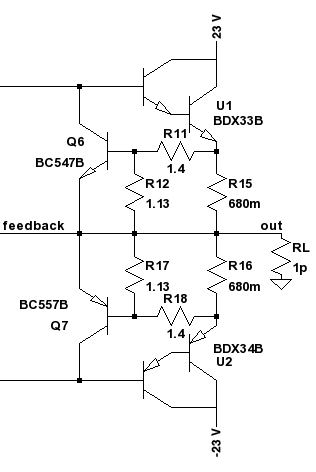
\includegraphics[scale=0.5]{teknisk/effektforstaerker/kortslut-done.png}
\caption{Kortslutningssikring indsat på udgangstrinnet}
\label{fig:kortslut-done}
\end{figure}

Kortslutningstrømmen var beregnet til 3 A, dog ses det på figur \ref{fig:kortslut-graf} at den negative halvperiode bliver begrænset ved omkring 2,8 A og den positive ved omkring 4,4 A.

\begin{figure}[h]
\centering
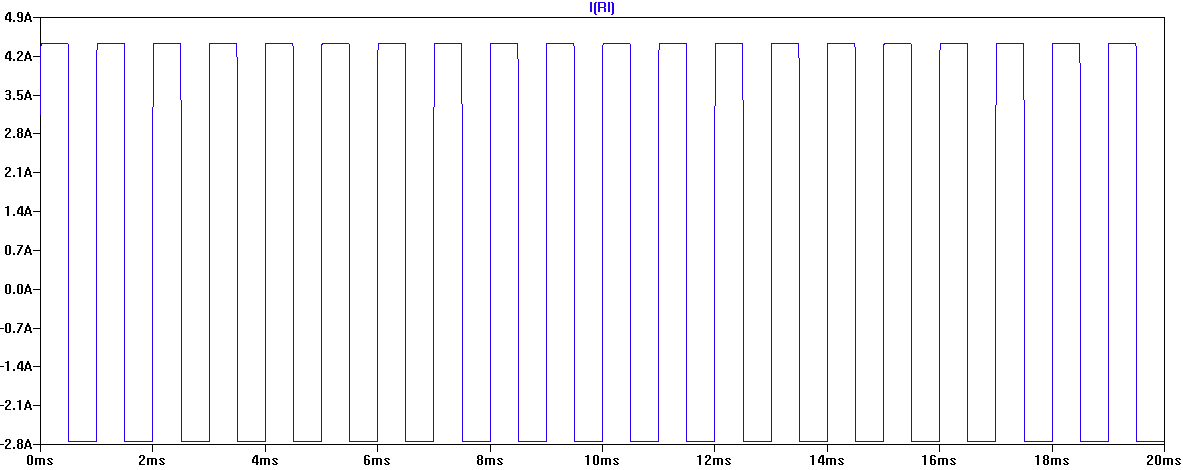
\includegraphics[width=\textwidth]{teknisk/effektforstaerker/kortslut-graf.png}
\caption{Graf over strømmen gennem belastningensmodstanden som repræsenterer en kortslutning}
\label{fig:kortslut-graf}
\end{figure}

Årsagerne til forskellene mellem de beregnede og simulerede værdier kan dog forklares. Ved den negative halvperiode antages det, at årsagen er at finde i at transistoren ikke behøver samme $V_\mathrm{be}$-spænding til at åbne som der er beregnet med, da denne værdi varierer fra transistor til transistor. Som det ses af udregningen i formel (\ref{equ:kortslut-vbe-test}) giver en strøm på 2,8 A en $V_\mathrm{be}$-spænding som ligger indenfor grænserne opgivet i databladet for BC557B \cite{bc557b-datablad}.%\kilde{BC557B.pdf}

\begin{equation}
\label{equ:kortslut-vbe-test}
1,13~\ohm \cdot \frac{\mathrm{680~m\ohm} \cdot \mathrm{2,8~A}}{1,4~\ohm + 1,13~\ohm + \mathrm{680~m\ohm}} = \mathrm{0,67~V}
\end{equation}

Forskellen i den positive halvperiode derimod antages at fremkomme ved at tilbagekoblingen forsøger at opretholde signalet på udgangen. Dette gør den ved at åbne mere for transistoren i spændingsforstærkeren, så der trækkes en større strøm i belastningen. Kortslutningsstrømmen kan fåes ned på 3 A, ved at ændre på modstandsværdierne hvis der insisteres på dette. 